\documentclass[12pt]{report}
\usepackage[dvipsnames]{xcolor}
\usepackage{amssymb,amsmath,graphicx}
\usepackage{hyperref}
\usepackage{tcolorbox}
\usepackage{tikz, appendix}
\usetikzlibrary{shapes,arrows}
\usetikzlibrary{calc}
\usetikzlibrary{positioning, decorations.pathmorphing, shadows,decorations.markings}
\usepackage{pgf,pgfarrows,pgfnodes,pgfautomata,pgfheaps,pgfshade,tikz}
\usepackage{soul}
\parindent=0pt
\parskip=4pt
\textwidth = 7in
\oddsidemargin = -.3in
\topmargin = -.8in
\textheight = 9.4in
\usepackage{empheq}
\usepackage{fontenc}
\usepackage{tikz}
\usepackage{pgfplots}
\usepackage{mathtools}
\usepackage{xfrac}
\usepackage{geometry}
\usepackage{xcolor}
\usepackage{physics}
\parindent=0pt
\parskip=16pt
\usepgfplotslibrary{fillbetween}
\newcommand*\widefbox[1]{\fbox{\hspace{2em}#1\hspace{2em}}}
\newcommand{\remarks}[1]{{\leavevmode\color{Aquamarine} #1}}
\newcommand{\examples}[1]{{\leavevmode\color{Maroon} #1}}
\newcommand{\definitions}[1]{{\leavevmode\color{blue} #1}}
\newcommand{\recap}[1]{{\leavevmode\color{teal} #1}}
\newcommand{\proof}[1]{{\leavevmode\color{ForestGreen} #1}}
\newcommand{\Mod}[1]{\(\mathrm{mod}\#1)}
\DeclareMathOperator{\rref}{rref}
\DeclareMathOperator{\nullity}{nullity}
\DeclareMathOperator{\Span}{Span}	
\DeclareMathOperator{\Nul}{Nul}
\parindent=0pt
\parskip=4pt
\textwidth = 7in
\oddsidemargin = -.3in
\topmargin = -.8in
\textheight = 9.4in
\begin{document}
	\begin{center} 
		\textbf{Math 171  \hfill  \textsc{Day 4- $\mathbb{Z}/n\mathbb{Z}$ and Intro to dihedral groups}\hfill Abstract Algebra}
		\rule{\linewidth}{.01in}
		\vskip 0.01in
	\end{center}
	\textsc{Professor Fukshansky}\\
	\vskip 0.05in
	\section{Recap}
	\recap{
	Let $(G,*)$ be a group. The \underline{order} of $G$ denoted $|G|$ is the number of elements in $G$. $|G|$ can be finite ($\mathbb{Z}/n\mathbb{Z}$ or $(\mathbb{Z}/n\mathbb{Z})^\times$) or infinite ($\mathbb{Z},\mathbb{Q}, \dots$). For finite groups, we often write $|G|<\infty$ and for infinite groups, we write $|G|=\infty$. 
	\vskip 0.05in
	If $x\in G$, then the order of $x$ denoted by $|x|$ is the \hl{smallest positive} integer $m$ such that $x^m=e$. If such an $m$ exists then we say that $|x|<\infty$ but if it doesn't we say that $|x|>\infty$. 
	}
	\vskip 0.05in
	\examples{
		\textbf{Example: } $2\in \mathbb{Z}/5\mathbb{Z}$ has an order of 5, but $2\in \mathbb{Z}$ has an infinite order because the identity is 0. 
	}
	\section{More on $\mathbb{Z}/n\mathbb{Z}$}
	\definitions{
	\textbf{Theorem: }Let $(G,*)$ be a group. If $x\in G$, $|x|\leq |G|$.
	}
	\vskip 0.05in
	\proof{
		The proof is based on the \underline{pidgeonhole principle} or the Dirichlet box principle: If there are $m$ objects placed into less than $n$ boxes, then there is a box with 2 or more objects. 
		\vskip 0.05in
		Since $G$ is a group and $x\in G$, all powers of $x\in G$. If $|G|=\infty$, ths already implies that $|x|\leq |G|$. However, if $|G|$ is finite, then $n=|G|$. Consider the elements $x,x^2,\dots,x^n,x^{n+1}\in G$.
		\vskip 0.05in
		$\therefore$ by the pidgeonhole principle, some $x^k=x^m$, with $1\leq k\leq m\leq n+1$. Then 
		$$x^k=x^m$$\\
		Multiplying the left sides of both sides of the equation by $x^{-1}$ $k$ times gives us $I_G=x^{m-k}$, with $1\leq m-k\leq n$. Therefore we have $|x|\leq m-k\leq n=|G|$. 
		}
	\vskip 0.1in
	\definitions{
		\textbf{Definition: }Let $(G,*)$ be a group such that $n=|G|<\infty$. Then $G=\{x_1,x_2,\dots,x_n\}$. A \hl{Multiplication table} for $G$ is defined as: 
		\begin{center}
			\begin{tabular}{|c|c|c|c|c|}
				\hline
				& $x_1$ & $x_2$ & $\dots$ & $x_n$ \\
				\hline
			$x_1$&  &        &         &       \\
			\hline
			$x_2$& & & & \\
			\hline
			$\dots$ & & & & \\
			\hline
			$x_n$ & & & &\\	
			\hline
			\end{tabular}
		\end{center}
	}
	\vskip 0.1in
	\examples{
		\textbf{Example: } Here is the multiplication table for $\mathbb{Z}/6\mathbb{Z}$
		\begin{center}
			\begin{tabular}{|c|c|c|c|c|c|c|}
				\hline 
				& 0 & 1 & 2 & 3 & 4 & 5\\
				\hline
				0 & 0 & 1 & 2 & 3 & 4 & 5\\
				\hline
				1 & 1 & 2 & 3 & 4 & 5 & 0\\
				\hline
				2 & 2 & 3 & 4 & 5 & 0 & 1\\
				\hline
				3 & 3 & 4 & 5 & 0 & 1 & 2\\
				\hline
				4 & 4 & 5 & 0 & 1 & 2 & 3\\
				\hline
				5 & 5 & 0 & 1 & 2 & 3 & 4\\
				\hline
			\end{tabular}
		\end{center}
		\textbf{Example: } Here is the multiplication table for $(\mathbb{Z}/8\mathbb{Z})^\times=\{1,3,5,7\}$
		\begin{center}
			\begin{tabular}{|c|c|c|c|c|}
				\hline
				& 1 & 3 & 5 & 7\\
				\hline
				1 & 1 & 3 & 5 & 7\\
				\hline
				3 & 3 & 1 & 7 & 5\\
				\hline
				5 & 5 & 7 & 1 & 3\\
				\hline
				7 & 7 & 5 & 3 & 1\\
				\hline
			\end{tabular}
		\end{center}
		\definitions{
		\fbox{Latin squares:}This happens when numbers appear but in different permutations. Every number appears. This is basically a sudoku grid. 
		}
	}
	\section{Intro to dihedral groups}
	\definitions{
		Let the dihedral group be the number of symmetries in a polygon. Let $P_n$ be a \hl{regular} polygon. That is, all sides are equal.
	}
	\vskip 0.05in
	\examples{ 
		\textbf{Example: }
		\vskip 0.025in
		This is $P_3$: 
		\begin{center}
		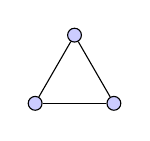
\begin{tikzpicture}[main_node/.style={circle,fill=blue!20,draw,minimum size=0.5em,inner sep=1pt}, every loop/.style={}]
			
			\node[main_node] (1) at (0, 0) {};
			\node[main_node] (2) at (0.5,0.8660254) {};
			\node[main_node] (3) at (1, 0) {};
			
			\path[every node/.style={}]
			(1) edge              node {} (2)
			(2) edge              node {} (3) 
			(3) edge              node {} (1);
		\end{tikzpicture}
		\end{center}
		\textbf{Example: }
		\vskip 0.025in
		This is $P_4$: 
		\begin{center}
			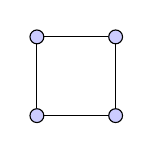
\begin{tikzpicture}[main_node/.style={circle,fill=blue!20,draw,minimum size=0.5em,inner sep=1pt}, every loop/.style={}]
				
				\node[main_node] (1) at (0, 0) {};
				\node[main_node] (2) at (0, 1) {};
				\node[main_node] (3) at (1, 1) {};
				\node[main_node] (4) at (1, 0) {};
				
				\path[every node/.style={}]
				(1) edge              node {} (2)
				(2) edge              node {} (3) 
				(3) edge              node {} (4)
				(4) edge              node {} (1);
			\end{tikzpicture}
		\end{center}
	}
	\vskip 0.1in
	\definitions{
	A rigid symmetry of $P_n$ is a transformation that maps $P_n$ onto itself. 
	}
	\vskip 0.05in
	\examples{
		\textbf{This is an example of a symmetry on $P_3$}:  
		\begin{center}
			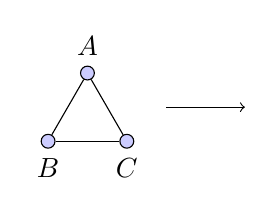
\begin{tikzpicture}[main_node/.style={circle,fill=blue!20,draw,minimum size=0.5em,inner sep=1pt}, every loop/.style={}]
				\node[main_node, label=below: $B$](1) at (0,0){};
				\node[main_node,label=below: $C$](2) at (1,0){};
				\node[main_node, label=above: $A$](3) at (0.5,0.8660254){};
				\path[every node/.style={}]
				(1) edge              node {} (2)
				(2) edge              node {} (3)
				(3) edge              node {} (1);
				\draw[->](1.5,0.433) -- (2.5,0.433);
			\end{tikzpicture}
			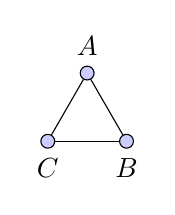
\begin{tikzpicture}[main_node/.style={circle,fill=blue!20,draw,minimum size=0.5em,inner sep=1pt}, every loop/.style={}]
				\node[main_node, label=below: $C$](1) at (0,0){};
				\node[main_node,label=below: $B$](2) at (1,0){};
				\node[main_node, label=above: $A$](3) at (0.5,0.8660254){};
				\path[every node/.style={}]
				(1) edge              node {} (2)
				(2) edge              node {} (3)
				(3) edge              node {} (1);
			\end{tikzpicture}
		\end{center}
	}
	\vskip 0.1in
	\definitions{
		\textbf{Definition:} \\
		We also have \hl{rotations}, where we rotate the shape $\frac{2\pi}{n}$ radians. 
	}	
	\vskip 0.05in
	\examples{
		\textbf{This is an example of a rotation on $P_3$}:
		\begin{center}
			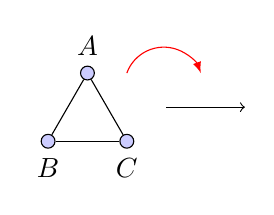
\begin{tikzpicture}[main_node/.style={circle,fill=blue!20,draw,minimum size=0.5em,inner sep=1pt}, every loop/.style={}]
				\node[main_node, label=below: $B$](1) at (0,0){};
				\node[main_node,label=below: $C$](2) at (1,0){};
				\node[main_node, label=above: $A$](3) at (0.5,0.8660254){};
				\path[every node/.style={}]
				(1) edge              node {} (2)
				(2) edge              node {} (3)
				(3) edge              node {} (1);
				\draw[-latex,red] ($(0.3,0.433)+(0.7,0.433)$) arc
				[
				start angle=160,
				end angle=20,
				x radius=0.5cm,
				y radius =0.5cm
				] ;
				\draw[->](1.5,0.433) -- (2.5,0.433);
			\end{tikzpicture}
			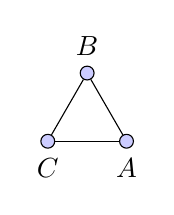
\begin{tikzpicture}[main_node/.style={circle,fill=blue!20,draw,minimum size=0.5em,inner sep=1pt}, every loop/.style={}]
				\node[main_node, label=below: $C$](1) at (0,0){};
				\node[main_node,label=below: $A$](2) at (1,0){};
				\node[main_node, label=above: $B$](3) at (0.5,0.8660254){};
				\path[every node/.style={}]
				(1) edge              node {} (2)
				(2) edge              node {} (3)
				(3) edge              node {} (1);
			\end{tikzpicture}
		\end{center}
	}
	\remarks{
		\textbf{Remarks: }For each $P_n$ we have the following symmetries: 
		\begin{itemize}
			\item \textbf{Rotations: } We can call a rotation from one shape to another a single ``click". There are a total of $n$ reflections because the first rotation is $\frac{2\pi}{n}$ radians, then the next one is $\frac{4\pi}{n}$ radians, and it stops when we get to the original shape when we rotate it $2\pi$ radians. 
			\item \textbf{Reflections: } There are $n$ reflections. As we can see in a triangle, there are 3 possible reflections. In a square there are 4 reflections. Using induction, in an $n$ gon there are $n$ reflections. 
		\end{itemize}
	}
	\vskip 0.1in
	\definitions{
	\textbf{Theorem: } A regular $n$-gon has precisely $2n$ symmetries. 
	}
	\vskip 0.05in
	\proof{
		\textbf{Proof: } Each symmetry is uniqule determined by where it sends a neighboring pair of vertices. Say vertices $A$ and $B$. Supose we want to send vertex $A$ to vertex $i$. Then $B$ goes to either $i+1$ or $i-1$. The total number of possibiliies for 1 neighboring verticie is $n$ so the total number of possiibiltiies for both neighboring verticies is $2n$.  
	}
	\vskip 0.1in
	\remarks{
		\textbf{Remarks: }The \underline{FULL} collection of symmetries of $P_n$ is: 
		\begin{itemize}
			\item $n$ symmetries
			\item $n$ reflections
		\end{itemize}
	}
	\vskip 0.1in
	\definitions{
		\textbf{Definition: } There are functions from $P_n\to P_n$. Define function composition as $\circ$ and $\sigma$ denotes a rotation and $\tau$ denotes a reflection. We can check that this is not a commutative operation: 
	}
	\vskip 0.05in
	\examples{
		\textbf{Example: }Let's say that we are in $P_4$ and that we want to find if $\tau\circ\sigma=\sigma\circ\tau$. Doing the left side we rotate first then find the reflection: 
		\begin{center}
			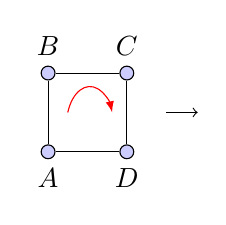
\begin{tikzpicture}[main_node/.style={circle,fill=blue!20,draw,minimum size=0.5em,inner sep=1pt}, every loop/.style={}]
				
				\node[main_node, label=below: $A$] (1) at (0, 0) {};
				\node[main_node, label=above: $B$] (2) at (0, 1) {};
				\node[main_node, label=above: $C$] (3) at (1, 1) {};
				\node[main_node, label=below: $D$] (4) at (1, 0) {};
				
				\path[every node/.style={}]
				(1) edge              node {} (2)
				(2) edge              node {} (3) 
				(3) edge              node {} (4)
				(4) edge              node {} (1);
				\draw[-latex,red] ($(0.25,0.25)+(0,0.25)$) arc
				[
				start angle=160,
				end angle=20,
				x radius=0.3cm,
				y radius =0.5cm
				] ;
				\draw[->] (1.5,0.5) -- (1.9,0.5);
			\end{tikzpicture}
			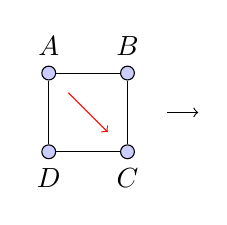
\begin{tikzpicture}[main_node/.style={circle,fill=blue!20,draw,minimum size=0.5em,inner sep=1pt}, every loop/.style={}]
				\node[main_node, label=below: $D$] (1) at (0, 0) {};
				\node[main_node, label=above: $A$] (2) at (0, 1) {};
				\node[main_node, label=above: $B$] (3) at (1, 1) {};
				\node[main_node, label=below: $C$] (4) at (1, 0) {};
				
				\path[every node/.style={}]
				(1) edge              node {} (2)
				(2) edge              node {} (3) 
				(3) edge              node {} (4)
				(4) edge              node {} (1);
				\draw[->,red](0.25,0.75) -- (0.75,0.25);
				\draw[->] (1.5,0.5) -- (1.9,0.5);
			\end{tikzpicture}
			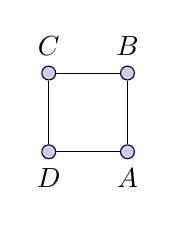
\begin{tikzpicture}[main_node/.style={circle,fill=blue!20,draw,minimum size=0.5em, inner sep=1pt}, every loop/.style={}]
				\node[main_node, label=below: $D$] (1) at (0, 0) {};
				\node[main_node, label=above: $C$] (2) at (0, 1) {};
				\node[main_node, label=above: $B$] (3) at (1, 1) {};
				\node[main_node, label=below: $A$] (4) at (1, 0) {};
				
				\path[every node/.style={}]
				(1) edge              node {} (2)
				(2) edge              node {} (3) 
				(3) edge              node {} (4)
				(4) edge              node {} (1);
			\end{tikzpicture}
		\end{center}
		The right most figure is what $\tau\circ\sigma$ is. Now evaluating the right side we get must find the reflection then rotate: 
		\begin{center}
			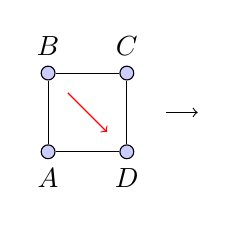
\begin{tikzpicture}[main_node/.style={circle,fill=blue!20,draw,minimum size=0.5em,inner sep=1pt}, every loop/.style={}]
				\node[main_node, label=below: $A$] (1) at (0, 0) {};
				\node[main_node, label=above: $B$] (2) at (0, 1) {};
				\node[main_node, label=above: $C$] (3) at (1, 1) {};
				\node[main_node, label=below: $D$] (4) at (1, 0) {};
				
				\path[every node/.style={}]
				(1) edge              node {} (2)
				(2) edge              node {} (3) 
				(3) edge              node {} (4)
				(4) edge              node {} (1);
				\draw[->,red](0.25,0.75) -- (0.75,0.25);
				\draw[->] (1.5,0.5) -- (1.9,0.5);
			\end{tikzpicture}
			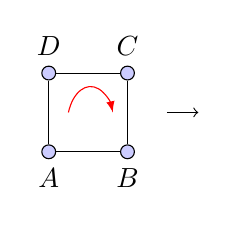
\begin{tikzpicture}[main_node/.style={circle,fill=blue!20,draw,minimum size=0.5em,inner sep=1pt}, every loop/.style={}]
				
				\node[main_node, label=below: $A$] (1) at (0, 0) {};
				\node[main_node, label=above: $D$] (2) at (0, 1) {};
				\node[main_node, label=above: $C$] (3) at (1, 1) {};
				\node[main_node, label=below: $B$] (4) at (1, 0) {};
				
				\path[every node/.style={}]
				(1) edge              node {} (2)
				(2) edge              node {} (3) 
				(3) edge              node {} (4)
				(4) edge              node {} (1);
				\draw[-latex,red] ($(0.25,0.25)+(0,0.25)$) arc
				[
				start angle=160,
				end angle=20,
				x radius=0.3cm,
				y radius =0.5cm
				] ;
				\draw[->] (1.5,0.5) -- (1.9,0.5);
			\end{tikzpicture}
			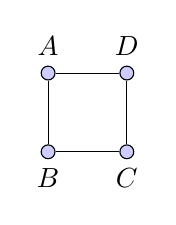
\begin{tikzpicture}[main_node/.style={circle,fill=blue!20,draw,minimum size=0.5em,inner sep=1pt}, every loop/.style={}]
				
				\node[main_node, label=below: $B$] (1) at (0, 0) {};
				\node[main_node, label=above: $A$] (2) at (0, 1) {};
				\node[main_node, label=above: $D$] (3) at (1, 1) {};
				\node[main_node, label=below: $C$] (4) at (1, 0) {};
				
				\path[every node/.style={}]
				(1) edge              node {} (2)
				(2) edge              node {} (3) 
				(3) edge              node {} (4)
				(4) edge              node {} (1);
			\end{tikzpicture}
		\end{center}
		The right most figure is what $\sigma\circ\tau$ is. Since the vertices are not in the same places, these two figures are not the same. We have shown that $\tau\circ\sigma\neq\sigma\circ\tau$. 
	}
\end{document}